% Options for packages loaded elsewhere
\PassOptionsToPackage{unicode}{hyperref}
\PassOptionsToPackage{hyphens}{url}
\PassOptionsToPackage{dvipsnames,svgnames,x11names}{xcolor}
%
\documentclass[
  letterpaper,
  DIV=11,
  numbers=noendperiod]{scrartcl}

\usepackage{amsmath,amssymb}
\usepackage{iftex}
\ifPDFTeX
  \usepackage[T1]{fontenc}
  \usepackage[utf8]{inputenc}
  \usepackage{textcomp} % provide euro and other symbols
\else % if luatex or xetex
  \usepackage{unicode-math}
  \defaultfontfeatures{Scale=MatchLowercase}
  \defaultfontfeatures[\rmfamily]{Ligatures=TeX,Scale=1}
\fi
\usepackage{lmodern}
\ifPDFTeX\else  
    % xetex/luatex font selection
\fi
% Use upquote if available, for straight quotes in verbatim environments
\IfFileExists{upquote.sty}{\usepackage{upquote}}{}
\IfFileExists{microtype.sty}{% use microtype if available
  \usepackage[]{microtype}
  \UseMicrotypeSet[protrusion]{basicmath} % disable protrusion for tt fonts
}{}
\makeatletter
\@ifundefined{KOMAClassName}{% if non-KOMA class
  \IfFileExists{parskip.sty}{%
    \usepackage{parskip}
  }{% else
    \setlength{\parindent}{0pt}
    \setlength{\parskip}{6pt plus 2pt minus 1pt}}
}{% if KOMA class
  \KOMAoptions{parskip=half}}
\makeatother
\usepackage{xcolor}
\setlength{\emergencystretch}{3em} % prevent overfull lines
\setcounter{secnumdepth}{-\maxdimen} % remove section numbering
% Make \paragraph and \subparagraph free-standing
\ifx\paragraph\undefined\else
  \let\oldparagraph\paragraph
  \renewcommand{\paragraph}[1]{\oldparagraph{#1}\mbox{}}
\fi
\ifx\subparagraph\undefined\else
  \let\oldsubparagraph\subparagraph
  \renewcommand{\subparagraph}[1]{\oldsubparagraph{#1}\mbox{}}
\fi


\providecommand{\tightlist}{%
  \setlength{\itemsep}{0pt}\setlength{\parskip}{0pt}}\usepackage{longtable,booktabs,array}
\usepackage{calc} % for calculating minipage widths
% Correct order of tables after \paragraph or \subparagraph
\usepackage{etoolbox}
\makeatletter
\patchcmd\longtable{\par}{\if@noskipsec\mbox{}\fi\par}{}{}
\makeatother
% Allow footnotes in longtable head/foot
\IfFileExists{footnotehyper.sty}{\usepackage{footnotehyper}}{\usepackage{footnote}}
\makesavenoteenv{longtable}
\usepackage{graphicx}
\makeatletter
\def\maxwidth{\ifdim\Gin@nat@width>\linewidth\linewidth\else\Gin@nat@width\fi}
\def\maxheight{\ifdim\Gin@nat@height>\textheight\textheight\else\Gin@nat@height\fi}
\makeatother
% Scale images if necessary, so that they will not overflow the page
% margins by default, and it is still possible to overwrite the defaults
% using explicit options in \includegraphics[width, height, ...]{}
\setkeys{Gin}{width=\maxwidth,height=\maxheight,keepaspectratio}
% Set default figure placement to htbp
\makeatletter
\def\fps@figure{htbp}
\makeatother
\newlength{\cslhangindent}
\setlength{\cslhangindent}{1.5em}
\newlength{\csllabelwidth}
\setlength{\csllabelwidth}{3em}
\newlength{\cslentryspacingunit} % times entry-spacing
\setlength{\cslentryspacingunit}{\parskip}
\newenvironment{CSLReferences}[2] % #1 hanging-ident, #2 entry spacing
 {% don't indent paragraphs
  \setlength{\parindent}{0pt}
  % turn on hanging indent if param 1 is 1
  \ifodd #1
  \let\oldpar\par
  \def\par{\hangindent=\cslhangindent\oldpar}
  \fi
  % set entry spacing
  \setlength{\parskip}{#2\cslentryspacingunit}
 }%
 {}
\usepackage{calc}
\newcommand{\CSLBlock}[1]{#1\hfill\break}
\newcommand{\CSLLeftMargin}[1]{\parbox[t]{\csllabelwidth}{#1}}
\newcommand{\CSLRightInline}[1]{\parbox[t]{\linewidth - \csllabelwidth}{#1}\break}
\newcommand{\CSLIndent}[1]{\hspace{\cslhangindent}#1}

\usepackage{booktabs}
\usepackage{caption}
\usepackage{longtable}
\usepackage{fontspec}
\usepackage{multirow}
\usepackage{multicol}
\usepackage{colortbl}
\usepackage{hhline}
\newlength\Oldarrayrulewidth
\newlength\Oldtabcolsep
\usepackage{array}
\usepackage{hyperref}
\usepackage{float}
\usepackage{wrapfig}
\usepackage{enumerate}
\KOMAoption{captions}{tableheading}
\makeatletter
\makeatother
\makeatletter
\makeatother
\makeatletter
\@ifpackageloaded{caption}{}{\usepackage{caption}}
\AtBeginDocument{%
\ifdefined\contentsname
  \renewcommand*\contentsname{Table of contents}
\else
  \newcommand\contentsname{Table of contents}
\fi
\ifdefined\listfigurename
  \renewcommand*\listfigurename{List of Figures}
\else
  \newcommand\listfigurename{List of Figures}
\fi
\ifdefined\listtablename
  \renewcommand*\listtablename{List of Tables}
\else
  \newcommand\listtablename{List of Tables}
\fi
\ifdefined\figurename
  \renewcommand*\figurename{Figure}
\else
  \newcommand\figurename{Figure}
\fi
\ifdefined\tablename
  \renewcommand*\tablename{Table}
\else
  \newcommand\tablename{Table}
\fi
}
\@ifpackageloaded{float}{}{\usepackage{float}}
\floatstyle{ruled}
\@ifundefined{c@chapter}{\newfloat{codelisting}{h}{lop}}{\newfloat{codelisting}{h}{lop}[chapter]}
\floatname{codelisting}{Listing}
\newcommand*\listoflistings{\listof{codelisting}{List of Listings}}
\makeatother
\makeatletter
\@ifpackageloaded{caption}{}{\usepackage{caption}}
\@ifpackageloaded{subcaption}{}{\usepackage{subcaption}}
\makeatother
\makeatletter
\@ifpackageloaded{tcolorbox}{}{\usepackage[skins,breakable]{tcolorbox}}
\makeatother
\makeatletter
\@ifundefined{shadecolor}{\definecolor{shadecolor}{rgb}{.97, .97, .97}}
\makeatother
\makeatletter
\makeatother
\makeatletter
\makeatother
\ifLuaTeX
  \usepackage{selnolig}  % disable illegal ligatures
\fi
\IfFileExists{bookmark.sty}{\usepackage{bookmark}}{\usepackage{hyperref}}
\IfFileExists{xurl.sty}{\usepackage{xurl}}{} % add URL line breaks if available
\urlstyle{same} % disable monospaced font for URLs
\hypersetup{
  pdftitle={Concept Mapping in Biology Education: A Systematic Review and Meta-Analysis},
  pdfauthor={Aaron Wenger},
  colorlinks=true,
  linkcolor={blue},
  filecolor={Maroon},
  citecolor={Blue},
  urlcolor={Blue},
  pdfcreator={LaTeX via pandoc}}

\title{Concept Mapping in Biology Education: A Systematic Review and
Meta-Analysis}
\author{Aaron Wenger}
\date{2023-09-21}

\begin{document}
\maketitle
\begin{abstract}
This is where the abstract will go
\end{abstract}
\ifdefined\Shaded\renewenvironment{Shaded}{\begin{tcolorbox}[sharp corners, frame hidden, interior hidden, boxrule=0pt, breakable, borderline west={3pt}{0pt}{shadecolor}, enhanced]}{\end{tcolorbox}}\fi

Concept mapping (CM) is an instructional activity invented in the 1970s
by Novak and his Cornell University research team (Novak \& Cañas,
2007). A concept map consists of conceptual nodes with connecting verbal
links (see Figure 1). Each node-link-node connection forms a
proposition. CM has been applied in a variety of ways and for a variety
of instructional purposes such as collaborative learning, group
discussion, directed reading, and formative assessment. With the move of
classes to online settings during the COVID-19 pandemic, CM has received
even more attention in science education as a tool for active learning
in virtual settings (Choe, 2020; Gerber Hornink \& Costa, 2021).

\begin{figure}

{\centering 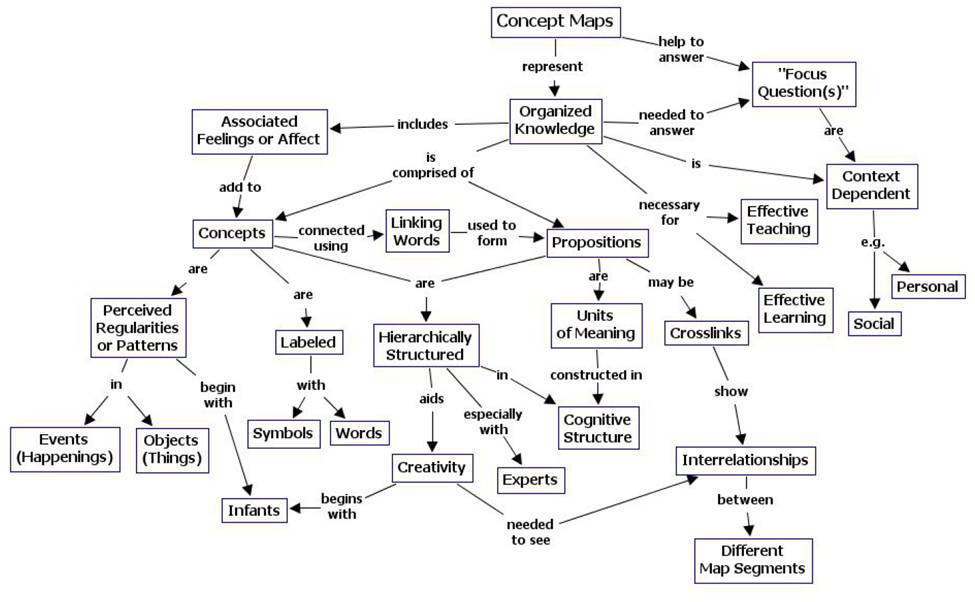
\includegraphics{example_concept_map.png}

}

\caption{An example concept map with its key features, from Novak \&
Cañas (2007)}

\end{figure}

Over the last 40 years, classroom intervention studies with CM have
proliferated and their results vary widely, often conflicting. Based on
the results of recent meta-analyses and reviews, it is apparent that
there is unexplained variance in the observed effects of CM in
instructional contexts. It is an open question whether some of this
variance is due to the influence of factors which affect the efficacy of
CM, of which we know little (Kinchin, 2014; Pudelko et al., 2012;
Schroeder et al., 2018), or other study-specific factors (e.g., study
design, comparison condition).

The present work is a systematic review and meta-analysis with the
primary purpose of learning more about the factors that influence the
effect size of CM interventions in empirical studies. As the use of CM
in education is a large, diverse, and complex topic, this project
focuses on CM use in biology education. The results are used to draw
conclusions on the efficacy of CM in biology education and to provide
guidance for future research.

\hypertarget{concept-mapping-in-context}{%
\section{Concept Mapping in Context}\label{concept-mapping-in-context}}

Proponents of various ``concept mapping'', ``mind mapping'', and
``knowledge mapping'' activities have promoted their innovations -- each
with some success -- to the education profession and the general public.
As a result, a confusion of terms has set in which creates difficulties
for research on CM (Åhlberg, 2004; Kinchin, 2014). The brief description
of CM given in the introduction -- as a diagram of conceptual nodes with
connecting verbal links -- serves as the definition of CM for this
project. In contrast, mind mapping is a simple association method
without a definitive structure or the use of verbal links (Åhlberg,
2004). Knowledge mapping is very similar to CM except that it uses a
definite set of terms for links between nodes (O'Donnell et al., 2001).

CM was developed by researchers as a means of representing children's
science knowledge (Novak \& Cañas, 2007) and has been used by
researchers in other contexts and applications as an instrument or
method. For example, CM has been used to measure conceptual change
(Wallace \& Mintzes, 1990) and as a method of planning program
evaluations (Trochim, 1989) and dissertation projects (Donnelly, 2017).
Early proponents of CM soon applied CM to instructional purposes as a
means of promoting Ausubel's meaningful learning construct via the
process of assimilation -- integration of new concepts into existing
conceptual frameworks (Novak \& Cañas, 2007).

The instructional uses of CM are varied. From the earliest years, CM was
recommended as a learning and formative assessment tool (J. Novak,
1981). Others applied CM as an advance organizer -- an overview of and
bridge between the student's prior knowledge and content to be learned
(Willerman \& Mac Harg, 1991). CM has been used in both a collaborative
group setting and with individual learners (Gao et al., 2007), with
students constructing their own maps or studying teacher-constructed
maps (Dyer et al., 2015). Lastly, CM has been applied extensively in
higher education (Kinchin, 2014), but also in K-12 schooling (Schroeder
et al., 2018).

While CM has been used as an instructive tool in many school subjects,
its first use was in biology education. The first article promoting the
instructional use of CM was published in The American Biology Teacher
(Stewart et al., 1979). Some researchers believe that CM can help
students summarize course content using the large vocabulary required in
introductory biology courses, thus promoting meaningful rather than rote
learning (Javonillo \& Martin-Dunlop, 2019). As stated by Schmid \&
Telaro (1990), ``Concept mapping \ldots{} appears to be ideally suited
to address biology content.'' (78-79).

\hypertarget{theoretical-framework-for-the-present-study}{%
\section{Theoretical Framework for the Present
Study}\label{theoretical-framework-for-the-present-study}}

Novak worked closely with David Ausubel and later with Bob Gowin (an
American philosopher of education at Cornell) coauthoring a book with
each (Ausubel et al., 1978; Novak \& Gowin, 1984). Ausubel proposed the
theory of meaningful learning which would later be closely associated
with schema theory and cognitive information processing (Driscoll,
2005). Gowin invented the Vee heuristic as a means of making knowledge
construction explicit, starting with objects/events and applying
concepts, theories, and practices to build up to knowledge claims (Novak
\& Gowin, 1984).

Concept mapping has either been framed as an implementation of either
cognitive information processing models or constructivist theories of
learning. Novak adopted his own subtype of constructivism, ``human
constructivism'', which was his attempt at unifying phenomena in
psychology and epistemology. In his first proposal of human
constructivism, Novak includes CM as a means of representing cognitive
structures and of demonstrating the constructivist process of learning
(Novak, 1993). In contrast, the work of Karpicke and colleagues has
considered CM as an elaborative encoding tool which may be effective to
the extent that memory is retrieved, processed in the mapping task, and
re-encoded (Blunt \& Karpicke, 2014; Karpicke \& Blunt, 2011).

The competing explanatory frameworks of Karpicke and Novak demonstrates
that there is room for differing interpretations of the efficacy of CM
and of relevant moderating factors. The present study adopts the
perspective of constructivism as this is the most prevalent theoretical
framework in CM intervention research. Novak and his colleagues consider
human constructivism to be a moderate epistemological position between
logical-positivism and social or radical constructivism (Mintzes et al.,
1998). They summarized it in three statements:

\begin{itemize}
\tightlist
\item
  Human beings are meaning makers.
\item
  The goal of education is to construct shared meanings.
\item
  The construction of shared meanings may be facilitated by
  well-prepared teachers.
\end{itemize}

\hypertarget{previous-meta-analyses}{%
\section{Previous Meta-Analyses}\label{previous-meta-analyses}}

A series of systematic reviews have examined the CM literature each with
a focus on a particular aspect or application of CM {[}e.g., Hartmeyer
et al. (2018), Machado \& Carvalho (2020), and Martin et al. (2015)). A
number of meta-analyses have also been conducted on the effects of CM
interventions. Most recently, Barta et al. (2022) synthesized the
metacognitive (i.e., critical thinking) and affective effects of CM
interventions across 21 studies. Yue et al. (2017) similarly synthesized
metacognitive effects but limited their scope to studies in medical
education. Erdoğan (2016) synthesized cognitive outcomes (i.e., learning
gains or academic achievement) but limited their scope to include only
studies in Turkey.

Nesbit \& Adesope (2006) have conducted the largest and most
comprehensive meta-analysis of cognitive and affective outcomes which
was updated in 2018 to include over 142 independent effect sizes (ES)
from 118 studies (Schroeder et al., 2018). They included all
experimental and quasi-experimental studies that contrasted CM with
other learning activities regardless of pedagogical setting or academic
discipline. Their analysis yielded an overall mean ES of 0.58 with an I2
of 87.5\%, after adjusting the value of two ES identified as outliers.
They conducted moderator analyses with five categorical variables using
the full set of independent effect sizes. They then divided the dataset
by CM type (constructed or studied) and conducted moderator analyses by
the four remaining variables plus three additional categorical
variables.

The largest differences in CM effects were seen for different comparison
conditions, region, and level of student interaction.\\
No other statistically significant and potentially meaningful
differences were seen except for duration of the intervention. The
results of the moderator analyses are shown in Table 1.

\setlength{\LTpost}{0mm}
\begin{longtable*}{l|l|cccc}
\caption*{
{\large Table 1} \\ 
{\small Moderator Analysis Results by CM Activity Type}
} \\ 
\toprule
\multicolumn{2}{l}{} & \multicolumn{2}{c}{Constructed} & \multicolumn{2}{c}{Studied} \\ 
\cmidrule(lr){3-4} \cmidrule(lr){5-6}
\multicolumn{2}{l}{Moderator} & k & g & k & g \\ 
\midrule
NA & Overall & 75 & 0.72 & 67 & 0.43 \\ 
\midrule
Comparison condition & Discussion/lecture & 32 & 1.05 & 5 & 1.09 \\ 
 & Studied or constructed lists & 0 & - & 13 & 0.43 \\ 
 & Studied or constructed outlines & 6 & 0.4 & 2 & 0.72 \\ 
 & Studied text & 5 & 0.33 & 39 & 0.29 \\ 
 & Constructed text & 10 & 0.48 & 3 & 0.1 \\ 
 & Other & 22 & 0.47 & 5 & 0.98 \\ 
\midrule
Academic discipline & STEM & 64 & 0.73 & 54 & 0.44 \\ 
 & non-STEM & 11 & 0.62 & 12 & 0.41 \\ 
 & Not reported & 0 & - & 1 & 0.05 \\ 
\midrule
CM mode & Interactive & 8 & 0.71 & 16 & 0.54 \\ 
 & Static & 66 & 0.72 & 39 & 0.4 \\ 
 & Animated & 0 & - & 7 & 0.47 \\ 
 & Mixed & 1 & 0.75 & 5 & 0.27 \\ 
\midrule
Intervention duration & <1 week & 14 & 0.4 & 33 & 0.34 \\ 
 & 1-4 weeks & 23 & 0.94 & 30 & 0.48 \\ 
 & >4 weeks & 37 & 0.72 & 4 & 0.7 \\ 
 & Unknown & 1 & 0.06 & 0 & - \\ 
\midrule
Country & Africa & 7 & 1.44 & 0 & - \\ 
 & Asia & 9 & 0.78 & 5 & 1.04 \\ 
 & Europe & 9 & 0.82 & 3 & 0.46 \\ 
 & Middle East & 13 & 0.75 & 2 & 0.96 \\ 
 & USA or Canada & 33 & 0.49 & 51 & 0.25 \\ 
 & Other/not reported & 4 & 0.62 & 6 & 1.29 \\ 
\midrule
School level & Intermediate & 22 & 0.68 & 7 & 0.82 \\ 
 & Secondary & 25 & 0.74 & 4 & 1.24 \\ 
 & Postsecondary and beyond & 28 & 0.73 & 56 & 0.32 \\ 
\midrule
Student interaction & In groups & 14 & 0.91 & 10 & 0.48 \\ 
 & Individual & 32 & 0.55 & 55 & 0.41 \\ 
 & Mixed & 22 & 0.91 & 0 & - \\ 
 & Other & 2 & 0.95 & 1 & 0.75 \\ 
 & Unknown & 5 & 0.29 & 1 & 0.47 \\ 
\bottomrule
\end{longtable*}
\begin{minipage}{\linewidth}
Results from Schroeder et al. (2018)\\
\end{minipage}

\hypertarget{potential-moderators-of-cm-efficacy}{%
\section{Potential Moderators of CM
Efficacy}\label{potential-moderators-of-cm-efficacy}}

In this section, the variables investigated in the present study are
described and related to Novak's human constructivism and other
considerations from the research synthesis literature. Variables were
sorted into four groups according to their significance to CM theory and
practice. This scheme was derived from the ideas of Lipsey (2019) and
the MUTOS framework of Becker (2017).

\hypertarget{extrinsic-characteristics}{%
\subsection{Extrinsic Characteristics}\label{extrinsic-characteristics}}

Extrinsic characteristics are those characteristics of included studies
which concern the researcher or research process. Differences in mean
effect sizes by publication status (i.e.~journal article or
dissertation/thesis) are known and described as a type of publication
bias (Cooper et al., 2019). In an empirical investigation of youth
psychotherapy trials, McLeod \& Weisz (2004) found that studies reported
in dissertations have a lower mean effect size than studies reported in
journal articles. Variation in publication year may be related to
characteristics of the methodology or intervention as practices have
evolved. It is likely that such variation exists given the age of CM
research as a research topic and instructional practices and so
publication year may moderate effects. The country or region where the
study was conducted is included as an extrinsic characteristic. While
the country or region where a study was conducted may serve as an
indicator of socio-cultural factors, it was judged that it is more
likely associated with extrinsic or methodological factors than
intervention or sample factors. Thus, region was included as an
extrinsic factor.

\hypertarget{methodological-characteristics}{%
\subsection{Methodological
Characteristics}\label{methodological-characteristics}}

In randomized controlled trials (RCTs) and quasi-experimental designs
(QEDs) a control or comparison condition is used to remove the influence
of factors unrelated to the treatment. Schroeder et al. (2018) coded a
variety of comparison conditions and concluded that larger CM effects
are associated with lecture and discussion comparisons as opposed to
various review activities such as creating or studying lists or texts.
It is possible that CM is both more effective than ``business-as-usual''
(BAU) methods -- such as lecturing -- and less effective than other
evidence-based methods -- such as retrieval practice (see Karpicke \&
Blunt, 2011).

A particular concern that some scholars have with studies using
experimental designs is that important contextual factors will be
controlled or ignored, thus leaving the researcher ignorant of their
importance to the CM intervention (Kinchin, 2014). Some studies take
place in a controlled laboratory setting (e.g., Karpicke \& Blunt, 2011)
while others assign whole course sections to each condition. In line
with general constructivist thought, CM proponents expect that findings
from laboratory settings will not generalize to classroom instruction,
perhaps underestimating the efficacy of CM (Mintzes et al., 2011; J. D.
Novak \& Gowin, 1984).

\hypertarget{intervention-characteristics}{%
\subsection{Intervention
Characteristics}\label{intervention-characteristics}}

CM interventions may require students to construct their own maps or
study map(s) constructed by the interventionist. Also, CM interventions
may involve interactive or animated maps facilitated by a digital CM
tool such as CmapTools (Cañas et al., 2004) or static maps created and
presented digitally or on a writing surface. While student construction
of concept maps is associated with larger effects, the mode of
implementation (interactive, animated, or static) is not associated with
different effects (Schroeder et al., 2018).

CM interventions where students construct maps may involve an initial
training period where students become familiar with the process as
recommended by CM proponents (Kinchin, 2011; Mintzes et al., 2011; J. D.
Novak \& Gowin, 1984). However, the extent of training may vary from
minutes to weeks (Karpicke \& Blunt, 2011b). It is not known what
effect, if any, that training has in CM efficacy.

The duration of CM interventions vary considerably from less than one
week to more than four weeks. In line with the importance of CM
training, some believe that CM interventions of a longer duration will
have more pronounced or long-lasting effects (Mintzes et al., 2011).
Schroeder et al.~(2018) concluded that longer intervention durations are
associated with larger effects.

Different strands of constructivism differ on the importance of student
social interaction in learning. It appears uncommon to directly examine
a CM condition with and without cooperative student interaction as
Okebuloa (1992) did or to state a clear rationale for designing an
intervention. Schroeder et al.~(2018) examined the level of
collaboration between learners as a moderator of CM efficacy and found
substantial differences between coded levels, though this was not
statistically significant.

\hypertarget{sample-characteristics}{%
\subsection{Sample Characteristics}\label{sample-characteristics}}

As mentioned above, CM has been applied at different grade levels,
across school subjects, and in varying contexts. A large majority of CM
research appears to have been conducted in STEM subjects rather than
non-STEM subjects, though there is no statistically significant or
meaningful difference between the two. Likewise, CM research has been
conducted across different grade levels. Per the conclusions of
Schroeder et al.~(2018), there doesn't seem to be a substantial or
statistically significant difference from intermediate to postsecondary
grade levels.

\hypertarget{rationale-and-research-questions}{%
\section{Rationale and Research
Questions}\label{rationale-and-research-questions}}

The work of Schroeder et al.~(2018) is excellent for its
contextualization of CM within educational theories and in its
discussion of theory vs.~evaluation-orientated research. However, it
falls short in its meta-analytic methods in important points. First, in
calculating effect sizes (ES) for studies with multiple CM conditions,
they calculated synthetic ESs which averaged the means and standard
deviations of each CM condition. In cases where outcome measures are
reported at multiple time points, Schroeder et al.~deferred to the last
measurement to calculate the ES. Both ES extraction decisions avoid
combining dependent ESs in the meta-analysis but at the cost of lower
statistical power, a lesser ability to explain heterogeneous effects,
and the potential for bias (COOPER, 2019). They can be avoided using
multilevel and/or multivariate meta-analyses (Tipton et al., 2019; Van
den Noortgate et al., 2015).

Second, Schroeder et al.~do not distinguish between cognitive and
affective (referred to as motivational) outcomes in their analysis.
Instead, they include both outcomes in a univariate meta-analytic model
which makes it difficult if not impossible to make meaningful
interpretations of their results. It is conceivable, if not probable,
that different socio-cultural and cognitive factors are important for
each outcome type. Also, the measures for each outcome type can be
expected to differ in important ways (e.g., recall or problem-solving
behavior vs.~self-report likert items). If these outcome types are to be
included in the same meta-analysis, each outcome could be analyzed
simultaneously using a multivariate model.

Third, Schroeder et al.~identified outliers using a formal method, but
one based on unweighted ES which does not take variances or the effect
of moderators into account. Smaller studies with larger variances may,
by chance, have large ES estimates and have little effect on estimation
of the meta-analytic model. Schroeder et al.~also did not examine these
identified outliers or conduct sensitivity analyses to determine the
robustness of their findings. Viechtbauer and Cheung (2010) recommend
the use of leave-1-out diagnostic statistics (such as studentized
deleted residuals or an analog of Cook's distances) to identify outliers
or influential cases and the use of sensitivity analyses in all
meta-analytic procedures.

Fourth, Schroeder et al.~used subgroup analysis to investigate all
moderators of CM effectiveness using only one variable (CM type) in
multi-way analyses, reexamining all other moderators. This causes three
problems: 1) inflated family-wise type I error, 2) no estimation of
residual or unexplained heterogeneity, and 3) an inability to conduct
statistical comparisons between moderators. It has long been known that
meta-regression using categorical covariates is equivalent to subgroup
analysis but also allows for residual heterogeneity to be estimated and
for statistical comparisons to be made (Thompson \& Higgins, 2002). As
recommended by Tipton, Pustejovsky, and Ahmadi (2019), meta-regression
models can include many moderator variables controlling family-wise type
I error and partialling out all moderator effects.

In this meta-analysis, these limitations were addressed using current
best practice in meta-analysis. The use of meta-regression with
multilevel-mixed-effects models containing relevant moderators allowed
the following research questions to be investigated:

\begin{enumerate}[{RQ}1.]
\item What is the mean effect size for CM interventions in biology education and to what extent does it vary within and between studies?
\item After controlling for study-level, extrinsic and methodological characteristics, to what extent does the mean effect size vary within and between studies?
\item What is the relationship between effect size and characteristics of the intervention and sample for CM interventions in biology education controlling for study-level, extrinsic and methodological characteristics?
\end{enumerate}

\hypertarget{methods}{%
\section{Methods}\label{methods}}

As with all systematic reviews, this study started with a systematic
literature search and screen for relevant records of research as defined
by criteria that addressed the research questions. These records and the
studies they reported were coded according to a prespecified scheme and
statistical information for ES calculation were extracted. The results
were then analyzed in multi-level, meta-regression models which took
into account the hierarchical structure of the data with multiple
effects often reported for each study. Influential cases were identified
and sensitivity analyses were conducted to check the robustness of the
results to them and to assumptions made during ES calculation. All
analyses were run in R () principally using the `metafor' () and
'clubSandwich` packages. All analysis code and meta-analysis data are
available at ---------.

\hypertarget{references}{%
\section*{References}\label{references}}
\addcontentsline{toc}{section}{References}

\hypertarget{refs}{}
\begin{CSLReferences}{1}{0}
\leavevmode\vadjust pre{\hypertarget{ref-AhlVarietiesConceptMapping2004}{}}%
Åhlberg, M. (2004). Varieties of {Concept Mapping}. \emph{Proceedings of
the First International Conference on Concept Mapping}, 4.

\leavevmode\vadjust pre{\hypertarget{ref-ANHEducationalPsychologyCognitive1978}{}}%
Ausubel, D. P., Novak, J. D., \& Hanesian, H. (1978). \emph{Educational
psychology: A cognitive view} (2d ed). {Holt, Rinehart and Winston}.

\leavevmode\vadjust pre{\hypertarget{ref-BFTSDevelopmentStudentsCritical2022}{}}%
Barta, A., Fodor, L. A., Tamas, B., \& Szamoskozi, I. (2022). The
development of students critical thinking abilities and dispositions
through the concept mapping learning method -- {A} meta-analysis.
\emph{Educational Research Review}, \emph{37}, 100481.
\url{https://doi.org/10.1016/j.edurev.2022.100481}

\leavevmode\vadjust pre{\hypertarget{ref-BecImprovingDesignUse2017}{}}%
Becker, B. J. (2017). Improving the {Design} and {Use} of {Meta
Analyses} in {Evidence-Based Practice}. In J. P. Sampson, E.
Bullock-Yowell, V. C. Dozier, D. S. Osborn, \& J. G. Lenz (Eds.),
\emph{Integrating {Theory}, {Research}, and {Practice} in {Vocational
Psychology}: {Current Status} and {Future Directions}}. {Florida State
University Libraries}. \url{https://doi.org/10.17125/svp2016.ch10}

\leavevmode\vadjust pre{\hypertarget{ref-BKLearningRetrievalbasedConcept2014}{}}%
Blunt, J. R., \& Karpicke, J. D. (2014). Learning with retrieval-based
concept mapping. \emph{Journal of Educational Psychology},
\emph{106}(3), 849--858. \url{https://doi.org/10.1037/a0035934}

\leavevmode\vadjust pre{\hypertarget{ref-ChoSynchronousCollaborativeOnline2020}{}}%
Choe, K. P. (2020). Synchronous and collaborative online concept mapping
of membrane transport. \emph{Biochemistry and Molecular Biology
Education}, \emph{48}(5), 516--517.
\url{https://doi.org/10.1002/bmb.21430}

\leavevmode\vadjust pre{\hypertarget{ref-CHVhrs2019}{}}%
Cooper, H. M., Hedges, L. V., \& Valentine, J. C. (Eds.). (2019).
\emph{Handbook of research synthesis and meta-analysis} (3rd Edition).
{Russell Sage Foundation}.

\leavevmode\vadjust pre{\hypertarget{ref-DonSystematicReviewConcept2017}{}}%
Donnelly, J. P. (2017). A systematic review of concept mapping
dissertations. \emph{Evaluation and Program Planning}, \emph{60},
186--193. \url{https://doi.org/10.1016/j.evalprogplan.2016.08.010}

\leavevmode\vadjust pre{\hypertarget{ref-DriPsychologyLearningInstruction2005}{}}%
Driscoll, M. P. (2005). \emph{Psychology of learning for instruction}
(3. ed). {Pearson Allyn and Bacon}.

\leavevmode\vadjust pre{\hypertarget{ref-DHM+ExamplebasedLearningComparing2015}{}}%
Dyer, J.-O., Hudon, A., Montpetit-Tourangeau, K., Charlin, B., Mamede,
S., \& Van Gog, T. (2015). Example-based learning: Comparing the effects
of additionally providing three different integrative learning
activities on physiotherapy intervention knowledge. \emph{BMC Medical
Education}, \emph{15}(1), 37.
\url{https://doi.org/10.1186/s12909-015-0308-3}

\leavevmode\vadjust pre{\hypertarget{ref-ErdInvestigationEffectivenessConcept2016}{}}%
Erdoğan, Y. (2016). An {Investigation} of the {Effectiveness} of
{Concept Mapping} on {Turkish Students}' {Academic Success}.
\emph{Journal of Education and Training Studies}, \emph{4}(6), 1--9.
\url{https://doi.org/10.11114/jets.v4i6.1380}

\leavevmode\vadjust pre{\hypertarget{ref-GSLTReviewStudiesCollaborative2007}{}}%
Gao, H., Shen, E., Losh, S., \& Turner, J. (2007). \emph{A {Review} of
{Studies} on {Collaborative Concept Mapping}: {What Have We Learned
About} the {Technique} and {What Is Next}?} 14.

\leavevmode\vadjust pre{\hypertarget{ref-GCConstructingOnlineConcept2021}{}}%
Gerber Hornink, G., \& Costa, M. J. (2021). Constructing online concept
maps in {CMap Cloud} collaboratively: {Connecting} pathways in case
scenarios. \emph{Biochemistry and Molecular Biology Education},
\emph{49}(1), 29--31. \url{https://doi.org/10.1002/bmb.21481}

\leavevmode\vadjust pre{\hypertarget{ref-HSBSystematicReviewConcept2018a}{}}%
Hartmeyer, R., Stevenson, M. P., \& Bentsen, P. (2018). A systematic
review of concept mapping-based formative assessment processes in
primary and secondary science education. \emph{Assessment in Education:
Principles, Policy \& Practice}, \emph{25}(6), 598--619.
\url{https://doi.org/10.1080/0969594X.2017.1377685}

\leavevmode\vadjust pre{\hypertarget{ref-JMLinkingPhrasesConcept2019}{}}%
Javonillo, R., \& Martin-Dunlop, C. (2019). Linking {Phrases} for
{Concept Mapping} in {Introductory College Biology}. \emph{Journal of
College Biology Teaching}, \emph{45}(3), 5.

\leavevmode\vadjust pre{\hypertarget{ref-KBRetrievalPracticeProduces2011a}{}}%
Karpicke, J. D., \& Blunt, J. R. (2011). Retrieval {Practice Produces
More Learning} than {Elaborative Studying} with {Concept Mapping}.
\emph{Science}, \emph{331}(6018), 772--775.
\url{https://doi.org/10.1126/science.1199327}

\leavevmode\vadjust pre{\hypertarget{ref-KinConceptMappingLearning2014}{}}%
Kinchin, I. M. (2014). Concept {Mapping} as a {Learning Tool} in {Higher
Education}: {A Critical Analysis} of {Recent Reviews}. \emph{The Journal
of Continuing Higher Education}, \emph{62}(1), 39--49.
\url{https://doi.org/10.1080/07377363.2014.872011}

\leavevmode\vadjust pre{\hypertarget{ref-LipIdentifyingPotentiallyInteresting2019}{}}%
Lipsey, M. W. (2019). Identifying {Potentially Interesting Variables}
and {Analysis Opportunities}. In H. M. Cooper, L. V. Hedges, \& J. C.
Valentine (Eds.), \emph{Handbook of research synthesis and
meta-analysis} (3rd Edition). {Russell Sage Foundation}.

\leavevmode\vadjust pre{\hypertarget{ref-MCConceptMappingBenefits2020}{}}%
Machado, C. T., \& Carvalho, A. A. (2020). Concept {Mapping}: {Benefits}
and {Challenges} in {Higher Education}. \emph{The Journal of Continuing
Higher Education}, \emph{68}(1), 38--53.
\url{https://doi.org/10.1080/07377363.2020.1712579}

\leavevmode\vadjust pre{\hypertarget{ref-MMSCriticalReviewConcept2015}{}}%
Martin, L. G., Martin, F. A., \& Southworth, E. (2015). A {Critical
Review} of {Concept Mapping Research Literature}: {Informing Teaching}
and {Learning Practices} in {GED Preparation Programs}. \emph{New
Horizons in Adult Education and Human Resource Development},
\emph{27}(3), 27--45. \url{https://doi.org/10.1002/nha3.20109}

\leavevmode\vadjust pre{\hypertarget{ref-MWude2004}{}}%
McLeod, B. D., \& Weisz, J. R. (2004). Using {Dissertations} to {Examine
Potential Bias} in {Child} and {Adolescent Clinical Trials}.
\emph{Journal of Consulting and Clinical Psychology}, \emph{72}(2),
235--251. \url{https://doi.org/10.1037/0022-006X.72.2.235}

\leavevmode\vadjust pre{\hypertarget{ref-MWNTeachingScienceUnderstanding1998}{}}%
Mintzes, J. J., Wandersee, J. H., \& Novak, J. D. (1998). \emph{Teaching
science for understanding: A human constructivist view}. {Academic
Press}.

\leavevmode\vadjust pre{\hypertarget{ref-NALearningConceptKnowledge2006a}{}}%
Nesbit, J. C., \& Adesope, O. O. (2006). Learning {With Concept} and
{Knowledge Maps}: {A Meta-Analysis}. \emph{Review of Educational
Research}, \emph{76}(3), 413--448.
\url{https://doi.org/10.3102/00346543076003413}

\leavevmode\vadjust pre{\hypertarget{ref-NovApplyingLearningPsychology1981}{}}%
Novak, J. (1981). Applying {Learning Psychology} and {Philosophy} of
{Science} to {Biology Teaching}. \emph{The American Biology Teacher},
\emph{43}(1), 12--42. \url{https://doi.org/10.2307/4447108}

\leavevmode\vadjust pre{\hypertarget{ref-NovHumanConstructivismUnification1993}{}}%
Novak, J. D. (1993). Human constructivism: {A} unification of
psychological and epistemological phenomena in meaning making.
\emph{International Journal of Personal Construct Psychology},
\emph{6}(2), 167--193. \url{https://doi.org/10.1080/08936039308404338}

\leavevmode\vadjust pre{\hypertarget{ref-NCtoc2007}{}}%
Novak, J. D., \& Cañas, A. J. (2007). Theoretical {Origins} of {Concept
Maps}, {How} to {Construct Them}, and {Uses} in {Education}.
\emph{Reflecting Education}, 15.

\leavevmode\vadjust pre{\hypertarget{ref-NGLearningHowLearn1984}{}}%
Novak, J. D., \& Gowin, D. B. (1984). \emph{Learning how to learn}.
{Cambridge University Press}.

\leavevmode\vadjust pre{\hypertarget{ref-ODHKnowledgeMapsScaffolds2001}{}}%
O'Donnell, A. M., Dansereau, D. F., \& Hall, R. H. (2001). Knowledge
{Maps} as {Scaffolds} for {Cognitive Processing}. \emph{Educational
Psychology Review}, 16.

\leavevmode\vadjust pre{\hypertarget{ref-PYVCMappingLearningStrategy2012a}{}}%
Pudelko, B., Young, M., Vincent-Lamarre, P., \& Charlin, B. (2012).
Mapping as a learning strategy in health professions education: A
critical analysis. \emph{Medical Education}, \emph{46}(12), 1215--1225.
\url{https://doi.org/10.1111/medu.12032}

\leavevmode\vadjust pre{\hypertarget{ref-STConceptMappingInstructional1990a}{}}%
Schmid, R. F., \& Telaro, G. (1990). Concept {Mapping} as an
{Instructional Strategy} for {High School Biology}. \emph{The Journal of
Educational Research}, \emph{84}(2), 78--85.
\url{https://doi.org/10.1080/00220671.1990.10885996}

\leavevmode\vadjust pre{\hypertarget{ref-SNAAStudyingConstructingConcept2018a}{}}%
Schroeder, N. L., Nesbit, J. C., Anguiano, C. J., \& Adesope, O. O.
(2018). Studying and {Constructing Concept Maps}: A {Meta-Analysis}.
\emph{Educational Psychology Review}, \emph{30}(2), 431--455.
\url{https://doi.org/10.1007/s10648-017-9403-9}

\leavevmode\vadjust pre{\hypertarget{ref-SVRcmt1979}{}}%
Stewart, J., Van Kirk, J., \& Rowell, R. (1979). Concept {Maps}: {A
Tool} for {Use} in {Biology Teaching}. \emph{The American Biology
Teacher}, \emph{41}(3), 171--175. \url{https://doi.org/10.2307/4446530}

\leavevmode\vadjust pre{\hypertarget{ref-TroIntroductionConceptMapping1989}{}}%
Trochim, W. M. K. (1989). An {Introduction} to {Concept Mapping} for
{Planning} and {Evaluation}. \emph{Evaluation and Program Planning},
\emph{12}, 1--16.

\leavevmode\vadjust pre{\hypertarget{ref-WMConceptMapResearch1990}{}}%
Wallace, J. D., \& Mintzes, J. J. (1990). The concept map as a research
tool: {Exploring} conceptual change in biology. \emph{Journal of
Research in Science Teaching}, \emph{27}(10), 1033--1052.
\url{https://doi.org/10.1002/tea.3660271010}

\leavevmode\vadjust pre{\hypertarget{ref-WMConceptMapAdvance1991}{}}%
Willerman, M., \& Mac Harg, R. A. (1991). The concept map as an advance
organizer. \emph{Journal of Research in Science Teaching}, \emph{28}(8),
705--711. \url{https://doi.org/10.1002/tea.3660280807}

\leavevmode\vadjust pre{\hypertarget{ref-YZZJEffectivenessConceptMapping2017}{}}%
Yue, M., Zhang, M., Zhang, C., \& Jin, C. (2017). The effectiveness of
concept mapping on development of critical thinking in nursing
education: {A} systematic review and meta-analysis. \emph{Nurse
Education Today}, \emph{52}, 87--94.
\url{https://doi.org/10.1016/j.nedt.2017.02.018}

\end{CSLReferences}



\end{document}
